\Tosca is a self-hosted, source-to-source compiler
generator. Its goal is to translate \Tosca programs to feature
rich programming languages such as \java, \cpp or \haskell---where the
current implementation genearates \java 8 programs. In this section,
we show the internals of \Tosca.
%
\Tosca works as a preprocessor. In other words: it does not rely
on a full compilation stack. As such, the \Tosca architecture 
is very simple, as depicted in Figure~\ref{fig:architecture}. This is because only features, and
associated lowerings~\cite{Bright:2014:Online} as well as optimizations,
present in \Tosca but not in the target language need
non-trivial translation.

To give an example: function closure, a common
feature found in many functional programming languages, including
\Tosca, is usually translated into a lower-level language using
 closure conversion~\cite{Johnsson85lambdalifting:}.  However since \java supports
closure---called anonymous class, or more recently \emph{lambda
  expressions} \cite{Gosling:2014:JLS:2462622}---\Tosca does not
need to apply this technique when translating to \java.
%
\newcommand*{\architecture}{%
  \begin{tikzpicture} [text height=1.5ex,text depth=.25ex]
    \node [block]                    (Parser) {Parser};
    \node [block, right = of Parser] (Normal) {Normalizer};
    \node [block, right = of Normal] (Specif) {Specifier};
    \node [block, right = of Specif] (CodeGe) {Code Generator};
    \path[->] (-2.5em, 0) edge (Parser)
              (Parser) edge (Normal)
              (Normal) edge (Specif)
              (Specif) edge (CodeGe) 
              (CodeGe) edge (23.5em, 0)
              ;
   \end{tikzpicture} 
}
%
\begin{figure}[h]
  \begin{center}
    \begin{tikzpicture}
      \node [fill=gray!20, draw] (greybox) {\architecture};
      \node at (13em,-1.5em)  (Cogs1) {\cogs{0.15}};
    \end{tikzpicture}
   \caption{The \Tosca Architecture.}
   \label{fig:architecture}
  \end{center}

\end{figure}

Going back to Figure~\ref{fig:use}, Figure~\ref{fig:architecture}
  shows what is happening inside the \Tosca compiler generator.
The \Tosca compilation phases---the Parser, Normalizer, Specifier,
and Code Generator---are described in details below.

Each compilation phase takes a (human) readable input and produces a
(human) readable output. Of course, some intermediate steps are
  easier to read than others, but we took a lot of effort to remain
  readable throughout. In particular, we find this important for the
  \java source code---i.e., the final output. This
approach is very advantageous for debugging and unit testing each compilation
phase individually. This is a common approach found in other compilers; \Tosca
systematizes it.

\subsection{Parser} \label{sec:parsing}
{
\renewcommand{\t}[1]{\ToscaIn{#1}}
\renewcommand{\a}[1]{\antlrIn{#1}}
% production
\newcommand{\p}[1]{\emph{#1}}
%
\begin{figure*}[!t]
      \begin{tabular}{l c p{6.7cm}}
      $\TG$⟦ \p{rule}$_1$ ... \p{rule}$_n$ ⟧  & = & $\TR$⟦ \p{rule}$_1$ ⟧ ... $\TR$⟦ \p{rule}$_n$ ⟧ \\[3pt] %  & (1) \\ 
      %
      $\TR$⟦ \a{NAME :} \p{alt} ⟧                 & = & \t{enum NAME(} $\TA$⟦ \p{alt} ⟧$_{NAME}$ \t{)}                              \\      %& (2) \\
      $\TR$⟦ \a{NAME :} \p{alt$_1$ ... alt$_n$} ⟧ & = &  \t{enum NAME} $\TA$⟦ \p{alt$_1$ ⟧$_{NAME_1}$ ... $\TA$⟦ alt$_n$ ⟧$_{NAME_n}$} \\[3pt] % & (3) \\
      %
      $\TA$⟦ \p{elmt}$_1$ ... \p{elmt}$_n$ ⟧$_{Name}$  & = & \t{| Name(} $\TE$⟦\p{elmt$_1$}⟧ ... $\TE$⟦ \p{elmt$_n$} ⟧ \t{)}  \\[3pt] %  & (4) \\
      %
      $\TE$⟦ \t{NAME}  ⟧                                  & = & \t{ NAME }                                      \\  % & (5) \\
      $\TE$⟦ \t{NAME} \p{ebnf} ⟧                          & = & \t{List( NAME )}                                \\  % & (6)\\
      $\TE$⟦ ( \p{elmt}$_1$ ... \p{elmt}$_n$ ) ⟧          & = & $\TE$⟦ \p{elmt}$_1$ ⟧ ... $\TE$⟦ \p{elmt}$_n$ ⟧  \\  % & (7) \\
      $\TE$⟦ ( \p{elmt}$_1$ ... \p{elmt}$_n$ ) \p{ebnf} ⟧ & = & $\TE$⟦ \a{ NAME } \p{ebnf} ⟧  \&
                                                                $\TR$⟦ \a{ NAME : } \p{elmt}$_1$ ... \p{elmt}$_n$ ⟧ \\  % & (8)\\
      $\TE$⟦ \t{NAME} \p{ebnf} \a{<bound=VARNAME>} ⟧      & = & $\mathcal{E}$                                         \\  % & (9) \\   
      $\TE$⟦ \t{NAME} \p{ebnf} \a{<boundvar=VARNAME>} ⟧   & = & [ \a{ NAME } ] \t{->} $\TE$⟦ \t{NAME} \p{ebnf} ⟧                      \\   % & (10) \\   
      $\TE$⟦ \t{NAME} \p{ebnf} \a{<symbol>} ⟧             & = & $\TE$⟦ \t{NAME} \p{ebnf} ⟧                          \\  % & (11) \\   
      $\TE$⟦ \t{NAME} \p{ebnf} \a{<sugar>} ⟧              & = & $\mathcal{E}$                                     \\  % & (12) 
      \end{tabular}
  \caption{Translating from the \antlr grammar to \Tosca types}
  \label{fig:parsing}
\end{figure*} 
}
The parser reads \Tosca program and produces an AST of the \Tosca 
program. This AST contains unparsed embedded program fragments, which are parsed 
during the normalization phase (cf. Section~\ref{sec:normalization}).
  
The current \Tosca implementation relies on the parser generator \antlr~v4~\cite{Parr:2013:DAR:2501720}
to represent both the \Tosca grammar and the embedded program grammars to be processed by \Tosca.
The choice of \antlr~v4 has mostly been driven by the following characteristics:
%
It has familiar EBNF-like notation making \antlr grammars easy to
write and read. Furthermore it has great support for automatic direct
left factoring and associativity, as well as a great performance
due to adaptive LL(*) parsing \cite{Parr:2014:ALP:2660193.2660202}.
Finally, it supports multiple target languages (e.g., \java, JavaScript) and 
it generates readable code, which is one of the priorities of \Tosca.
%
All this fits very well in the \Tosca philosophy of ease-of-use, 
without compromising functionality and performance. 

\Tosca is able to handle programs written in different languages by defining common \emph{mapping rules}
from \antlr grammar concepts to \Tosca typed expression.
These mapping rules are fundamental for implementing several tools 
provided by \Tosca including the
\begin{enumerate*} [label=\itshape(\roman*)]
  \item \Tosca parser,
  \item parsers for the embedded program fragments, and also
  \item a \Tosca type description corresponding to \Tosca
    expressions recognized by these parsers.
\end{enumerate*}
%
Figure~\ref{fig:parsing} shows these mapping rules for the following
simplified grammar of \antlr itself:
%
\begin{lstANTLR}
  grammar     : rule* 
  rule        : NAME : alt* 
  alt         : elmt*
  elmt        : NAME ebnf? option? | block ebnf?
  block       : ( alt* ) 
  ebnf        : '?' | '*' | '+'
  option      : <sugar> | <bound=VARNAME> 
              | <boundvar=VARNAME> | <symbol>   
\end{lstANTLR}

As seen before, an \antlr grammar consists of a set of \emph{grammar rules}. Each
rule is identified by an unique \antlrIn{NAME}, and defines a list of \emph{alternatives} (\antlrIn{alt}).
Each alternative is defined as sequence of \emph{elements} (\antlrIn{elmt}) composing it, which in turn
corresponds to \emph{token} of a given \antlrIn{NAME} and \antlrIn{block}.  

The mapping of \antlr grammar onto \Tosca is shown in Figure~\ref{fig:parsing}. The mapping rules are 
of the form 
\begin{center}
  $\T_{\subsT{rulename}}$⟦\antlr⟧ =  \ToscaIn{Tosca type},
\end{center}
 where $\T_{\subsT{rulename}}$ ($\T$ for $\T\textit{ranslation}$) is a function on an \antlr construct, 
\emph{rulename} is one of the \antlr grammar rule names given above and \antlrIn{NAME} an environment containing the current 
alternative name (see below).  

Each grammar \emph{rule} is translated into a \Tosca enumeration of the corresponding 
rule name. For a grammar rule with only a single alternative, the alternative name is set to the name
of the rule. Otherwise the alternative name is set to the rule name suffixed by the alternative position in the rule.
A rule reference becomes an enumeration value. Repetition, either \emph{zero or one element}~(\antlrIn{'?'}), \emph{zero or more elements}~(\antlrIn{'*'}) 
or \emph{one or more elements}~(\antlrIn{'+'}), maps to list of values. While this mapping is approximate, it has the advantage of being compatible with the 
\Tosca standard library operating on lists (cf.~Section~\ref{sec:forreal}). 
A block with repetition cannot be mapped directly to a \Tosca enumeration. \Tosca eliminates blocks
by lifting the block elements to a top level grammar rule 
(The 3rd and 4th rule of $\TE$). The $\&$ symbol indicates an additional type is created. Elements with the option \antlrIn{<sugar>}
are filtered out during parsing and therefore do not appear in \Tosca (as represented by $\mathcal{E}$).    

The parser turns \antlr events into \Tosca expressions following the type mapping rules. The only difficulty
comes from handling scoped variables. It works as follows: custom actions are added to the \antlr grammar to indicate which
event corresponds to either a bound variable (\antlrIn{<boundvar>}), the beginning and the end of a scope (\antlrIn{<bound>}),
or to a variable occurrence (\antlrIn{<symbol>}). These action allows the parser to internally keep track of in-scope variables
needed to create bindings upon variable occurrences. If binding creation fails, i.e., no variable is found in the in-scope variables,
a fresh variable is created. 

\subsection{Normalizer} \label{sec:normalization}

The normalizer turns the AST with embedded program fragments and
syntactic sugar, as produced by the parser, into \Tosca Core.
The formal description is presented in
Section~\ref{sec:coretotransscript}---here we give the implementation
details.

The main task performed by the normalizer is to expand embedded
program fragments into \Tosca and then \Tosca Core, as
shown in Example~\ref{ex:embedinline} and
Example~\ref{ex:expandinline} in Section~\ref{sec:language}.

A further task is to translate syntactic sugar constructs into their
core representation equivalent.  In both tasks it is important to
preserve the original program location to produce high-fidelity error
messages by showing \Tosca program snippets written by
programmers.

The normalizer relies on \emph{meta parsers} to parse the embedded
programs, which are derived from \emph{meta grammars}.
%
\begin{definition} \label{metaGrammar} %
  A \emph{meta grammar} is a grammar that has been augmented with
  additional rules to be able to:
  \begin{enumerate*} [label=\itshape(\roman*)]
  \item embed \Tosca expressions in places where terminals and non-terminals occur,
  \item directly declare meta variables in the rule's left-hand side 
and reference them in the rule's right-hand side, and 
  \item parse program fragments, delimited by a grammar rule.
  \end{enumerate*}
\end{definition}

\Tosca is capable of automatically generating meta grammars from a
given grammar.  A snippet of the generated grammar for \MiniML is
shown in Example~\ref{ex:minimlgrammar}---and for the bootstrapping we
also generated a meta grammar for the \Tosca language
itself~(cf.~Section~\ref{sec:forreal}).  This is accomplished as
follows:
\begin{itemize}
\item Each grammar rule corresponds to two meta grammar rules: the first
  one matches the original grammar rule with some extensions, and the
  second one, which by convention is suffixed by \ToscaIn{_EOF},
  allows the grammar rule to represent the whole program.
\item Two alternatives are added to each grammar rule: one to parse
  meta variables (in the meta grammar), and the other to escape back to the \Tosca
  program. By default, meta variable tokens are prefixed by the
  character \ToscaIn{#}. In case of conflict with the target 
  language, another character can be chosen.
\item Embedded \Tosca programs are read as a single stream of
  characters (a token), which is fed to the \Tosca parser to
  produce the AST. The AST is recursively normalized, which in turn can
  trigger subsequent parsing and normalization translations. This recursive process
  stops when the AST contains no more embedded code.
\end{itemize}

\begin{example} \label{ex:minimlgrammar}
  The meta grammar corresponding to the \ToscaIn{toplevel} and
  \ToscaIn{expr} grammar rules from Example~\ref{ex:MiniML}
  is given next:
%
\begin{lstANTLR}
toplevel_EOF : toplevel EOF 

toplevel : 'let' var_TOK  '=' expr ';' toplevel ';;'
         |  expr  ';;'
         |  '#toplevel' 
         | ET_toplevel
             
var_TOK_EOF : var_TOK EOF

var_TOK : VAR  | '#VAR' 
         | ET_var_TOK

expr_EOF :  expr EOF  

expr : timesExpr '+' expr  
      | timesExpr '-' expr
      | timesExpr 
      | '#expr' 
      | ET_expr  

// Lexer rules

ET_toplevel: '⟨toplevel:' -> pushMode(Embed);
ET_var_TOK : '⟨VAR:' -> pushMode(Embed); 
ET_expr: '⟨expr:' -> pushMode(Embed); 

mode Embed ;    
EMBED_END   : '⟩' -> popMode;
EMBED_NESTED: '⟨' -> pushMode(NestedEmbed), more; 
EMBEDDED    : . -> more;  

mode NestedEmbed;  
NESTED_EMBED_END   : '⟩' -> popMode, more;  
NESTED_EMBED_NESTED: '⟨' -> pushMode(NestedEmbed), more;
NESTED_EMBEDDED    : . -> more; 
\end{lstANTLR}	
\end{example}

This example clearly shows the \antlrIn{_EOF} grammar rules, as well
as the additional rule alternatives explained above. Parsing embedded
\Tosca code is done by defining two special lexer modes,
\antlrIn{Embed} and \antlrIn{NestedEmbed} allowing nesting.

After normalization is done, the AST contains only \Tosca Core
and is ready for the specificity phase.

\subsection{Specifier} \label{specification} \label{sec:specification}

A very reasonable expectation of a programming language is that it is
deterministic. But term rewriting stems from equational
reasoning---and not programming. Thus, as opposed to (functional)
programs, term rewrite systems are not deterministic \emph{per se}. 
%
\begin{example} \label{ex:div}
 We want to implement integer division and start with the
 following three rules. 
 %
\begin{lstTosca}
rule Div(0, #Y) → 0
rule Div(#X, 0)  → NaN
rule Div(#X, #Y) → Plus(1, Div(Minus(#X, #Y), #Y))
 \end{lstTosca}
 % 
 But if we now consider the term \ToscaIn{Div(0,0)}, three
 different rewrite steps are possible:
 \begin{center}	
   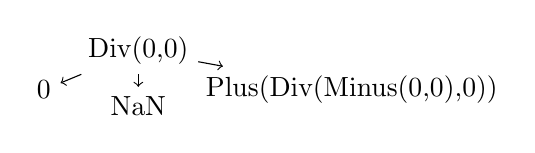
\begin{tikzpicture}[node distance=2em]
      \node (1)  {\ToscaIn{Div(0,0)}};
      \node (2) [below left of = 1, xshift=-2em] {\ToscaIn{0}}; 
      \draw[->] (1) -- (2);
      \node (3) [below right of = 1, xshift=6.3em]{\ToscaIn{Plus(Div(Minus(0,0),0))}}; 
      \draw[->] (1) -- (3);
      \node (4) [below of =  1] {\ToscaIn{NaN}};
      \draw[->] (1) -- (4);
    \end{tikzpicture}
  \end{center}  
\end{example}
%
Now the task of the \emph{specifier} is to resolve such an ambiguous
situation based on specificity criteria. While this phase is not
strictly needed in the basic \Tosca architecture, it is a unique
feature rarely found in other programming languages and therefore
presented here---but not yet fully integrated in the compilation
phases.
%
So why does this problem occur in the first place? Because the three
rules \emph{overlap} (cf.~Section~\ref{sec:CRS}).
%
In particular, we have an overlap between the
first two rules with %
%
\ToscaIn{#X} $\mapsto$ \ToscaIn{0} and
\ToscaIn{#Y} $\mapsto$ \ToscaIn{0} %
%
and the second and third rule with %
 \ToscaIn{#Y} $\mapsto$ \ToscaIn{0}.
%

So how to disambiguate this situation? In Example~\ref{ex:div} we may
observe that there are different kinds of overlaps.
%
If we look at the overlap between the second and third rule, we see
that one is more \emph{specific} than the other. That is,
\ToscaIn{Div(#X, 0)} is an instance of
\ToscaIn{Div(#X,#Y)}. It is reasonable to assume that the
third rule is conceived as the ``fallback'' rule by the programmer.

But between the first and the second rule we have a completely
ambiguous situation---and in fact, we chose to inform the programmer
of this ambiguity, i.e., we raise an exception.

Following \cite{1990_kennaway}, we take this as a basis for
disambiguation through specificity: We build a
\emph{specificity tree}.
%
\begin{example} 
For the following four terms
\begin{lstTosca}
  Div(#X, #Y), Div(0, #Y), Div(0, 0), Div(NaN, #Y)
\end{lstTosca}  
we can build the specificity tree, where the corresponding $\sigma$s are
given on the edges.
\begin{center}	  
  \begin{tikzpicture}[node distance=8mm]
    \node (1)                                  {\ToscaIn{Div(#X, #Y)}};
    \node (2) [below left of = 1, xshift=-5em] {\ToscaIn{Div(0, #Y)}};
    \draw[->] (1) -- node[above left]  {\ToscaIn{\#X} $\mapsto$ \ToscaIn{0}} (2);
    \node (3) [below right of = 1, xshift=5em] {\ToscaIn{Div(NaN, #Y)}}; 
    \draw[->] (1) -- node[above right]         {\ToscaIn{\#X} $\mapsto$ \ToscaIn{NaN}}    (3);
    \node (4) [below of =  2]                  {\ToscaIn{Div(0,0)}};
    \draw[->] (2) -- node[left]                {\ToscaIn{\#Y} $\mapsto$ \ToscaIn{0}}   (4);
  \end{tikzpicture}
\end{center} 
%
But if we additionally add \ToscaIn{Div(#X, 0)}, we have a
parallel overlap, i.e., a situation which cannot be handled by
specificity. 
%
\end{example}
%
By applying the rule in post order with respect to the specificity
tree, we try the most specific rule first. That is, we have the rules
ordered by specificity---or an error if it is non-solvable: a parallel
overlap.  Compared to, e.g., \cite{2007_maranget}, we may relate the
following concepts: a set of rewrite rules is completely defined iff
it is exhaustive. A pattern is useless, if there is a (non-parallel)
overlap.

The specificity tree, as presented, can serve for several analyses and
transformations. For example, we can use the tree to figure out
whether a function symbol is completely defined. Or, we may transform
the rules by instantiating less specific rules and thereby remove
overlaps---an approach currently taken by \crsx~\cite{2011_rose}. 

In particular the following result helps for disambiguation.  Recall,
that \Tosca rules are left-linear
(cf. Section~\ref{sec:CRStocore}).  Thus an application of
Theorem~\ref{t:1} yields confluence, as soon as we can guarantee that
the rules are non-overlapping.

So far, we presented why we need the specifier and the potentials of
the specificity tree. But how do we actually find overlaps?  To detect
them, we implement \emph{higher-order unification for patterns}. This
implementation is based on \cite[Figure~2]{1993_nipkow}, and presented
here briefly.  The following example is suitably adapted from
Nipkow~\cite{1993_nipkow}.

\begin{example} 
%
  As an illustrative example we show how to compute $\sigma$ between
  the two concrete terms:
%
 \ToscaIn{F(#X, [x y] -> #F(x))} and %
 \ToscaIn{F(0, [x y] -> C(#G(y x)))}.
%
 So we give intermediate steps in \Tosca syntax (or multiple
 steps denoted by $\to^*$). The function \ToscaIn{Unify} takes a
 \ToscaIn{Pair} of terms and a $\sigma$, which is empty
 (\ToscaIn{ \{\} }) at the beginning.
%
\begin{lstTosca}
Unify(Pair(F(#X, [x y] -> #F(x)), 
            F(0,  [x y] -> C(#G(y x)))), {}) 
↠ If(ConstructorEqual(F,F), 
     Foldl([args sigma] -> Unify(args, sigma), {}, 
           (Pair(#X, 0),
            Pair([x y] -> #F(x), [x y] -> C(#G(y,x)))
\end{lstTosca}
To \ToscaIn{Unify} the two terms we first compare their root
symbols. As they are both constructors and equal, we proceed to
\ToscaIn{Foldl} over the arguments. To unify the first pair of
arguments is straightforward.
%
\begin{lstTosca}
rule Unify(Pair(#X, 0), {}) ↠ { #X ↦ 0 }
\end{lstTosca}
%
To unify those two terms, we have to map the meta variable
\ToscaIn{#X} to the term \ToscaIn{0}.
%
The next pair of arguments is more involved as it contains functions.
%
\begin{lstTosca}
Unify(Pair([x y] -> #F(x)), [x y] -> C(#G(y, x))), {}) 
↠ Unify(Pair(#F(x), C(#G(y,x))), {})
\end{lstTosca}
%
We can strip away the variables \ToscaIn{x y}, as they are equal. In
general, we have to deal here with implementing $\alpha$-conversion.
%
\begin{lstTosca}
↠ Unify(Pair(#H(x), #G(y,x)), {#F ↦ [x] -> C(#H(x))})
\end{lstTosca}
%
In this step, we have to introduce a fresh meta variable
\ToscaIn{#H}. We map the meta variable \ToscaIn{#F} to a
function, which takes one argument \ToscaIn{x} and starts with
the function symbol~\ToscaIn{C}, which has a argument our fresh
meta variable \ToscaIn{#H} with one argument---as
\ToscaIn{#F}.
%
For the last step, i.e., unifying \ToscaIn{Pair(#H(x),
  #G(y,x))}, we have to identify the two meta
variables~\ToscaIn{#H} and \ToscaIn{#G}. Therefore, we map
them both to a fresh meta variable \ToscaIn{#H2}.
%
\begin{lstTosca}
↠ { #H ↦ [x] -> #H2(x), #G ↦ [y x] -> #H2(x),
       #F ↦ [x] -> C(#H2(x))} 
\end{lstTosca}
%
We have to make sure, to also apply \ToscaIn{#H ↦ [x] -> #H2(x)}
to the image of \ToscaIn{#F}.
\end{example}
%
\subsection{Code Generator} \label{sec:codegen}

Finally the last compilation phase is the code generator producing human
readable \java source code. The generated code relies on a common 
runtime \java library providing the following capabilities:
%
\begin{enumerate*} [label=\itshape(\roman*)]
\item \label{cap:fun} A generic way to represent terms. \Tosca functions and enumerations share the same
generic term representation, with the 
only difference that functions are associated 
with a generated \java method corresponding to the function rules. 
\item A substitution algorithm which traverses the term tree to look
  for bound variable occurrences, and substitutes them by other terms.
\item A top level normalization algorithm that repeatedly attempts to
  reduce the outermost functional term until there are none, or the
  reduction is stuck.
\item A way to pretty print terms to a generic term format. 
\item A way to construct terms. 
\end{enumerate*}

As mentioned in Capability~\ref{cap:fun} for 
each \Tosca function corresponds to a single \java method that 
has the following structure:
\begin{itemize}
\item Each \Tosca function's rule corresponds a \java labeled block---in the same lexical order.
\item The first part of the \java labeled block encodes the
  rule's left hand side. It checks for construction symbols and
  associates meta variables to terms.  If the pattern matching fails,
  a break command is issued to jump to the next \java block.
\item The rule contraction is generated in the second part of the \java labeled block. A new term is generated by 
using a combination of new term construction, associated meta variables, and substitution.
\end{itemize}
%
\begin{example} \label{ex:code}
The \java code corresponding to MiniML \ToscaIn{EvalExpr} is the following one:
\begin{lstTosca}
static Boolean evalExpr(Sink sink, Term term) {
  if (sink.context().sd++ < 256) 	{
			rule1 : {
				term = force(sink.context(), term);
				if (term.descriptor() != MiniML_xexpr_xA1)
					break rule1;
				Term sub0 = term.sub(0).ref();
				/* #timesExpr=sub0 */
				Term sub1 = term.sub(1).ref();
				/* #expr=sub1 */
				sink.start(Plus);
				sink.start(EvalTimesExpr);
				sink.copy(sub0.ref());
				sink.end();
				sink.start(EvalExpr);
				sink.copy(sub1.ref());
				sink.end();
				sink.end();
				return true;
			}
			rule2 : { ... }
			rule3 :	{ ... }
		}
		return thunk(sink, evalExpr, term);
	}	
\end{lstTosca}
\end{example} 
%
The most important characteristics of the \java code in
Example~\ref{ex:code} are the following ones: The test in line 2 makes
sure the stack does not overflow. It relies on a common known technique
called \emph{trampoline}. When the stack depth reaches an arbitrary
threshold (there is no way to know the \java max stack depth), the
method evaluation is interrupted and a corresponding thunk is returned
in line 24. Here, the Boolean value indicates, whether we have a failed or a successful step.
The first rule starts at line 3, the second rule and third are
sketched in line 21 and 22. Then,
\ToscaIn{force} evaluates a term enough to be in head normal
form---as can be seen in line~4. Line~5 corresponds to the
beginning of pattern matching and line 7 is the beginning of the
right-hand side rules.

%%% Local Variables:
%%% mode: latex
%%% TeX-master: "techreport"
%%% End:
